%%%
%%% FORMAL GAP IDENTIFICATION
%%%
\section{Deriving the Gap to Ordinary Transformation}

\mnote{Gap between synchronizing and ordinary transformations}
We have introduced that there is both a formal and a practical gap between synchronizing transformations, which we have defined as a component of transformation networks, and ordinary transformations, which are unidirectional and non-synchronizing as used by many transformation languages.
In the following, we first give an example for faulty behavior if we simply used ordinary transformations in a transformation network.
Afterwards, we give a formal definition of unidirectional preservation rules and ordinary transformations, then defined as \emph{bidirectional transformations}.
Finally, we discuss the relation between unidirectional consistency preservation rules and unidirectional consistency relations, as introduced in \autoref{chap:correctness:finegrained}.

%%
%% MOTIVATING FAULT EXAMPLE WITH ORDINARY TRANSFORMATIONS
%%
%\subsection{Behavior of Ordinary Transformations in Networks}

\mnote{Failure in motivational example}
We have already sketched the example of creating a class in \gls{UML} and Java after adding a component to a \gls{PCM} model in \autoref{chap:introduction:challenges:correctness:synchronization}.
In that scenario, it was possible that for a created \gls{PCM} component first a \gls{UML} class is generated, which is then transformed into a Java class.
Additionally, the transformation between \gls{PCM} and Java creates another Java class, as it does not consider that there may be another transformation that has already created that class.
Such scenarios can lead to the duplication of elements, as an already existing element is inserted again, or to an overwrite of an already existing element.
Overwriting a previously created element may also remove information that was already added to it, like the transformation across \gls{UML} may have added information to the Java class which is overwritten by the class creation of the transformation from \gls{PCM} to Java.

\mnote{Failure in running example}
An analogous example can be given for the running example of persons, employees, and residents depicted in \autoref{fig:networks:three_persons_example}.
We consider the consistency relations $\consistencyrelation{CR}{PE}, \consistencyrelation{CR}{ER}$, and $\consistencyrelation{CR}{PR}$.
As discussed in \autoref{chap:compatibility}, these relations are compatible, thus for any given person, employee, or resident, there is a consistent tuple of models containing it.
Thus, the relations do not prevent transformations from finding consistent models whenever a person, employee or resident is added.
Ordinary transformations with unidirectional consistency preservation rules react to the changes in one model and update another accordingly.
In case of adding a person, this may look as depicted in \autoref{fig:synchronization:duplicate_creation_example}.
For each of the given consistency relations, we assume unidirectional consistency preservation rules that preserve consistency according to them.
They especially create an employee for each added person and a resident for each created employee and person, respectively.
Since the transformations assume the models to be consistent before applying the changes, they always add a corresponding element when one of the elements is added.
This leads to the situation that the consistency preservation rules for both $\consistencyrelation{CR}{PR}$ as well as $\consistencyrelation{CR}{ER}$, namely $\consistencypreservationrule{\consistencyrelation{CR}{PR}}$ and $\consistencypreservationrule{\consistencyrelation{CR}{ER}}$, create a resident upon creation of a person.
In consequence, there exist two residents with the same $\mathvariable{name}$, which does not fulfill the consistency relations.

\begin{figure}
    \centering
    \newcommand{\hdistance}{16.5em}
\newcommand{\vdistance}{8em}
\newcommand{\objectwidth}{6.8em}

\begin{tikzpicture}[
    consistency preservation/.style={-latex, consistency changed element, font=\small},
    user change/.style={-latex, user changed element, font=\small},
]

\umlobjectvarwidth[, fill=white]{person}{}{
: Person}{
firstname = "Alice"
lastname = "Avid"
}{\objectwidth}

\umlobjectvarwidth[, fill=white, right=\hdistance of person.north, anchor=north] {employee}{}{
: Employee}{
name = "Alice Avid"
}{\objectwidth}

\umlobjectvarwidth[, fill=white, below=\vdistance of employee.north, anchor=north] {resident1}{}{
: Resident}{
name = "Alice Avid"
}{\objectwidth}

\umlobjectvarwidth[, fill=white, left=0.5*\hdistance of resident1.north, anchor=north] {resident2}{}{
: Resident}{
name = "Alice Avid"
}{\objectwidth}

\umlhuman{human}{at ([xshift=-0.55*\hdistance]person.center)}{}{}{0.5}
\draw[user change] (human) -- node[above, align=center] {\guillemotleft creates \guillemotright} (human.east-|person.west);
\draw[consistency preservation] (person.east|-employee.west) -- node[above] {created by $\consistencypreservationrule{\consistencyrelation{CR}{PE}}$} (employee.west);
\draw[consistency preservation] (employee.south) -- node[left] {created by $\consistencypreservationrule{\consistencyrelation{CR}{ER}}$} (resident1.north);
\draw[consistency preservation] (person1.south) |- node[below, pos=0.5] {created by $\consistencypreservationrule{\consistencyrelation{CR}{PR}}$} (resident2.west);

\end{tikzpicture}


    %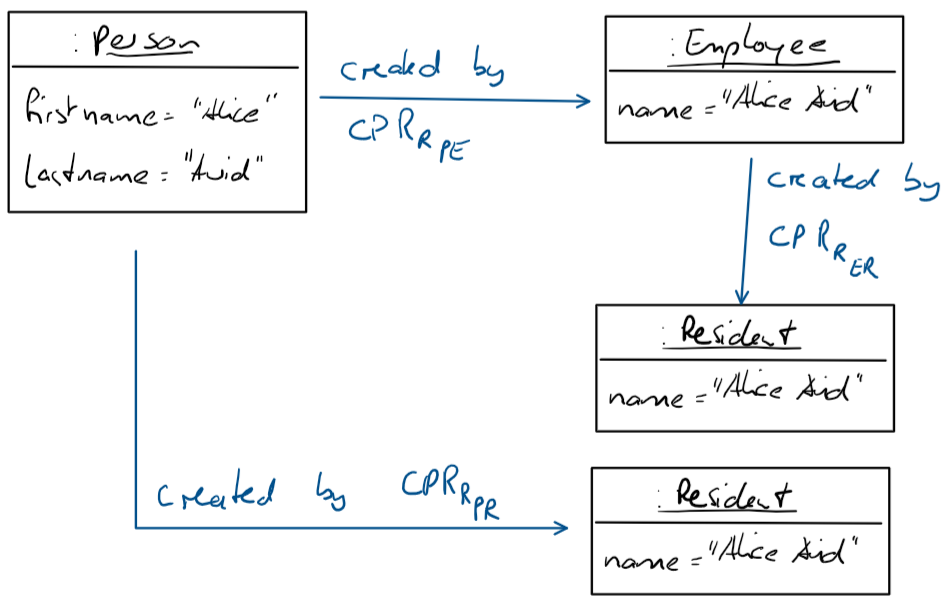
\includegraphics[width=0.8\textwidth]{figures/correctness/synchronization/duplicate_creation_example.png}
    \caption[Duplicate creation of an element]{Duplicate creation of a resident by two sequences of consistency preservation rules.}
    \label{fig:synchronization:duplicate_creation_example}
\end{figure}

\mnote{Avoidance of failures}
It is our goal to find out how such a situation can be avoided by proper definition of consistency preservation rules in existing transformation languages.
A simple solution in this example would have been to first check whether the elements to create already exist.
This can either be done by using a trace model, which many transformation language use to store corresponding elements, or by searching for an appropriate element in the other model, using some key information like its name.
Using a trace model, however, has some drawbacks and pitfalls, which we investigate in \autoref{chap:synchronization:achieving:identification}.


%%
%% UNIDIRECTIONAL CONSISTENCY PRESERVATION RULES
%%
\subsection{Unidirectional Consistency Preservation Rules}

\mnote{Unidirectional preservation rules}
Before we can discuss options how unidirectional consistency preservation rules can be used to emulate the behavior of synchronizing consistency preservation rules, we first need to define them to be able to formally compare the two of them.
In contrast to a synchronizing consistency preservation rule as defined in \autoref{def:consistencypreservationrule}, a unidirectional consistency preservation rule only receives changes made to one of the two models and returns changes to the other model instead of receiving and returning changes to both.

\begin{definition}[Unidirectional Consistency Preservation Rule]
    \label{def:unidirectionalconsistencypreservationrule}
    Let $\consistencyrelationset{CR}$ be a set of consistency relations between elements of two metamodels $\metamodel{M}{1}$ and $\metamodel{M}{2}$.
    A \emph{unidirectional consistency preservation rule} $\consistencypreservationrule{\consistencyrelationset{CR}}$ for the relation set $\consistencyrelationset{CR}$ is a partial function:
    \ifisafour\else\vspace{-0.3em}\fi
    \begin{align*}
        \consistencypreservationrule{\consistencyrelationset{CR}} : (\metamodelinstanceset{M}{1}, \metamodelinstanceset{M}{2}, \changeuniverse{\metamodel{M}{1}}) \rightarrow \changeuniverse{\metamodel{M}{2}} \cup \setted{\bot}
    \end{align*}
\end{definition}

\mnote{Preservation rules in transformation languages}
This is how the consistency preservation rules defined in or derived from many existing transformation languages operate.
They take two models and changes to one of them and generate changes for the other.
Most of them even directly apply the changes instead of returning a dedicated change artifact.
The rule is partial to indicate inputs of models and changes that it is not able to handle. In these cases, the function returns $\bot$.

\mnote{Correctness of unidirectional preservation rules}
In addition, these rules usually expect the input models to be consistent and then ensure that after applying the input and the output changes to the models, the resulting models are consistent again.
Their behavior for inconsistent input models is undefined, such that they either return $\bot$ or a change that does not necessarily guarantee that the models are consistent after applying the input and output changes.
This conforms to the common notion of \emph{correctness} for consistency preservation rules, like for the state-based (rather than our delta-based) notion of consistency preservation rules defined by \textcite{stevens2010sosym}.
This is even compliant to the correctness notion that we have defined for synchronizing consistency preservation rules in \autoref{def:consistencypreservationrulecorrectness}.
Thus, we define correctness of a unidirectional consistency preservation rule as follows.

\begin{definition}[Unidirectional Preservation Rule Correctness]
    \label{def:unidirectionalconsistencypreservationrulecorrectness}
    Let $\consistencypreservationrule{\consistencyrelationset{CR}}$ be a unidirectional consistency preservation rule.
    We call $\consistencypreservationrule{\consistencyrelationset{CR}}$ \emph{correct} if, and only if, the resulting models when applying the input and output changes are consistent to $\consistencyrelationset{CR}$ again:
    \ifisafour\else\vspace{-0.3em}\fi
    \parameterizeformat{
    \begin{align*}
        &
        \consistencypreservationrule{\consistencyrelationset{CR}} \correctmath \equivalentperdefinition 
        \forall 
        \model{m}{1} \in \metamodelinstanceset{M}{1}, 
        \model{m}{2} \in \metamodelinstanceset{M}{2},
        \change{\metamodel{M}{1}} \in \changeuniverse{\metamodel{M}{1}} : \\
        & \formulaskip
        \big[ \tupled{\model{m}{1}, \model{m}{2}} \consistenttomath \consistencyrelationset{CR} \Rightarrow
            #2
            \forall 
            \change{\metamodel{M}{2}} \in \changeuniverse{\metamodel{M}{2}} :
            \big( 
                \consistencypreservationrule{\consistencyrelation{CR}{}}(\model{m}{1}, \model{m}{2}, \change{\metamodel{M}{1}}) = \change{\metamodel{M}{2}}
                #1 #2 \formulaskip
                \Rightarrow
                \tupled{\change{\metamodel{M}{1}}(\model{m}{1}), \change{\metamodel{M}{2}}(\model{m}{2})} \consistenttomath \consistencyrelationset{CR} 
            \big)
        \big]
    \end{align*}
    }{\\ & \formulaskip}{\\ & \formulaskip\formulaskip}%
\end{definition}

\mnote{Optional partiality of synchronizing preservation rules}
In \autoref{def:unidirectionalconsistencypreservationrule}, we explicitly allow consistency preservation rules to be partial.
This was only an optional requirement for synchronizing consistency preservation rules defined in \autoref{def:consistencypreservationrule}, because there may be changes to both models that cannot be processed reasonably as one of the changes may need to be reverted to achieve consistency.
Ignoring this practical requirement, it is theoretically possible to always return changes that, if applied to the input models, produce consistent models.
These changes may perform arbitrarily unreasonable modifications but still restore consistency.

\mnote{Mandatory partiality of unidirectional preservation rules}
For unidirectional consistency preservation rules, partiality is not only a practical requirement.
They must be partial, because there can be models for which no other models can be generated such that they are consistent to a consistency relation set.
Consider the consistency relation $\consistencyrelation{CR}{} = \setted{\tupled{a, z}, \tupled{b, z}}$ and its transposed $\consistencyrelation{CR}{}^T = \setted{\tupled{z, a}, \tupled{z, b}}$.
If a change led to the model $\model{m}{} = \setted{a, b}$, then no second model to which it is consistent can be generated.
A consistent model would have to contain $z$, because $\consistencyrelation{CR}{}$ requires for $a$ and $b$ an element $z$ to exist in another model.
$\consistencyrelation{CR}{}^T$, however, requires that for a $z$ only either $a$ or $b$ exists in the other model, as otherwise no witness structure with unique corresponding elements can be found (see \autoref{def:consistency}).
In consequence, a unidirectional consistency preservation rule cannot produce a result for such an input without violating the correctness definition.

\mnote{Undefined behavior}
In fact, the definition does not specify for which inputs a unidirectional consistency preservation rule is allowed to be undefined.
One could restrict this behavior to cases in which there is no $\change{\metamodel{M}{2}} \in \changeuniverse{\metamodel{M}{2}}$ for given models $\model{m}{1}$ and $\model{m}{2}$ and a given change $\change{\metamodel{M}{1}} \in \changeuniverse{\metamodel{M}{1}}$ such that $\tupled{\change{\metamodel{M}{1}}(\model{m}{1}), \change{\metamodel{M}{2}}(\model{m}{2})} \consistenttomath \consistencyrelationset{CR}$ for consistency relations $\consistencyrelationset{CR}$.
We, however, leave it up to the developer to decide for which inputs a consistency preservation rule is undefined, as there might be cases in which a change restoring consistency can theoretically be generated but does semantically not make sense.
This was also the reason for allowing a synchronizing consistency preservation rule to be partial, which is why we have already discussed the scenario in \autoref{chap:correctness:formalization:incremental_inductive}.


%%
%% NONALIGNMENT OF UNIDIRECTIONAL CONSISTENCY RELATIONS AND UNIDIRECTIONAL CONSISTENCY PRESERVATION RULES
%%
\subsection{Unidirectional Relations and Preservation}
\label{chap:synchronization:gap:alignment}

\mnote{Unidirectional preservation rules for unidirectional relations}
Because of the definition of unidirectional consistency preservation rules based on a unidirectional notion of consistency relations, it seems reasonable to have a unidirectional consistency preservation rule associated with the unidirectional consistency relations for one direction between two metamodels.
For each pair of metamodels, this would result in two sets of unidirectional consistency relations and a consistency preservation rule for each of them.

\begin{figure}
    \centering
    \newcommand{\classwidth}{5.2em}
\newcommand{\objectwidth}{5.2em}
\newcommand{\hdistance}{(19.3em+0.5*\difftoafiveimage)}
\newcommand{\vdistance}{19em}

\begin{tikzpicture}

\umlclassvarwidth{employee_class}{}{Employee}{
    name
}{\classwidth}
\umlclassvarwidth[, right=1.4*\hdistance of employee_class.north west, anchor=north]{resident_class}{}{Resident}{
    name
}{\classwidth}

\draw[directed consistency relation]
    (employee_class)
    --
    node[pos=0, above right] {$e$}
    node[pos=1, above left] {$r$}
    node[above] {$\consistencyrelation{CR}{ER} = \setted{\tupled{e,r} \mid \mathvariable{e.name} = \mathvariable{r.name}}$}
    node[below, align=center] {$\consistencyrelation{CR}{ER}' = \consistencyrelation{CR}{ER} \; \cup $ \\ $\setted{\tupled{e,r} \mid \mathvariable{e.name} = \mathvariable{r.name.toLower}}$}
    (resident_class);

% FIRST SCENARIO
\coordinate (begin_first) at ([yshift=-0.25*\vdistance]employee_class.north west);
\draw[lightgray] (begin_first) -- (begin_first-|resident_class.east);
\node[anchor=north west] at ([yshift=-0.5em]begin_first) {1. Removing an employee with $\consistencypreservationrule{\consistencyrelation{CR}{ER}}$ only for $\consistencyrelation{CR}{ER}$};

\umlobjectvarwidth[, below right=0.18*\vdistance and 0.45*\hdistance of begin_first, anchor=north]{employee_first}{}{: Employee}{
    name = "Alice"
}{\objectwidth}
\umlobjectvarwidth[, right=0.95*\hdistance of employee_first.center, anchor=center]{resident_first}{}{: Resident}{
    name = "Alice"
}{\objectwidth}
\node[below=0.4*\vdistance of employee_first.north, anchor=north] (non_employee_first) {$\emptyset$};

\draw[consistency execution]
    ([xshift=-0.3*\hdistance]employee_first.west)
    --
    node[above, align=center] {1.\\ add by user}
    (employee_first.west);
\draw[consistency execution]
    ([yshift=0.5em]employee_first.east)
    --
    node[above] {2. add by $\consistencypreservationrule{\consistencyrelation{CR}{ER}}$}
    ([yshift=0.5em]resident_first.west);
\draw[correspondence]
    ([yshift=-0.5em]employee_first.east)
    --
    node[below] {consistent to $\setted{\consistencyrelation{CR}{ER}, \consistencyrelation{CR}{ER}^T}$}
    ([yshift=-0.5em]resident_first.west);
\draw[consistency execution]
    (employee_first)
    --
    node[left, align=center] {3.\\ remove by user}
    (non_employee_first);
\draw[correspondence]
    (non_employee_first)
    --
    node[above, pos=0.35, sloped] {consistent to $\consistencyrelation{CR}{ER}$}
    node[below, pos=0.35, sloped] {inconsistent to $\consistencyrelation{CR}{ER}^T$}
    ([xshift=2em]resident_first.south west);

% SECOND SCENARIO
\coordinate (begin_second) at ([yshift=-0.7*\vdistance]begin_first);
\draw[lightgray] (begin_second) -- (begin_second-|resident_class.east);
\node[anchor=north west] at ([yshift=-0.5em]begin_second) {2. Adding a resident with its effect to $\consistencyrelation{CR}{ER}'$};

\umlobjectvarwidth[, below=0.18*\vdistance of begin_second, anchor=north west]{employee_second}{}{: Employee}{
    name = "alice"
}{\objectwidth}
\umlobjectvarwidth[, right=0.95*\hdistance of employee_second.center, anchor=center]{resident1_second}{}{: Resident}{
    name = "alice"
}{\objectwidth}
\umlobjectvarwidth[, below=0.2*\vdistance of resident1_second.center, anchor=center]{resident2_second}{}{: Resident}{
    name = "Alice"
}{\objectwidth}

\draw[consistency execution]
    ([xshift=0.3*\hdistance]resident2_second.east)
    --
    node[below] {add by user}
    (resident2_second.east);
\draw[correspondence]
    ([yshift=0.5em]employee_second.east)
    --
    node[above] {consistent to $\consistencyrelation{CR}{ER}'$}
    ([yshift=0.5em]resident1_second.west);
\draw[correspondence]
    ([yshift=-0.5em]employee_second.east)
    --
    ([yshift=-0.5em]resident1_second.west);
\coordinate (cross_second) at ([yshift=-0.5em]$(employee_second.east)!0.75!(resident1_second.west)$);
\draw[correspondence]
    (cross_second)
    |-
    node[pos=0.25, left, align=center] {inconsistent\\ to $\consistencyrelation{CR}{ER}'$}
    (resident2_second);
\filldraw[consistency related element] (cross_second) circle (0.15em);


% THIRD SCENARIO
\coordinate (begin_third) at ([yshift=-0.6*\vdistance]begin_second);
\draw[lightgray] (begin_third) -- (begin_third-|resident_class.east);
\node[anchor=north west] at ([yshift=-0.5em]begin_third) {3. Removing an employee with its effect to $\consistencyrelation{CR}{ER}'$};

\umlobjectvarwidth[, below right=0.18*\vdistance and 0.5*\hdistance of begin_third, anchor=north]{employee1_third}{}{: Employee}{
    name = "alice"
}{\objectwidth}
\umlobjectvarwidth[, draw=lightgray, text=gray, below=0.2*\vdistance of employee1_third.center, anchor=center]{employee2_third}{}{: Employee}{
    name = "Alice"
}{\objectwidth}
\umlobjectvarwidth[, right=0.9*\hdistance of employee1_third.center, anchor=center]{resident1_third}{}{: Resident}{
    name = "alice"
}{\objectwidth}
\umlobjectvarwidth[, below=0.2*\vdistance of resident1_third.center, anchor=center]{resident2_third}{}{: Resident}{
    name = "Alice"
}{\objectwidth}

\draw[consistency execution]
    ([xshift=-0.3*\hdistance]employee2_third.west)
    --
    node[above, align=center] {remove\\ by user}
    (employee2_third.west);
\draw[correspondence]
    ([yshift=0.5em]employee1_third.east)
    --
    node[above] {inconsistent to $\consistencyrelation{CR}{ER}'$}
    ([yshift=0.5em]resident1_third.west);
\coordinate (cross_thirdupper) at ([yshift=0.5em]$(employee1_third.east)!0.6!(resident1_third.west)$);
\draw[correspondence]
    (cross_thirdupper)
    |-
    ([yshift=0.5em]resident2_third.west);
\filldraw[consistency related element] (cross_thirdupper) circle (0.15em);
\draw[correspondence]
    ([yshift=-0.5em]employee2_third.east)
    --
    node[below] {consistent to $\consistencyrelation{CR}{ER}'$}
    ([yshift=-0.5em]resident2_third.west);
\coordinate (cross_thirdlower1) at ([yshift=-0.5em]$(employee2_third.east)!0.25!(resident2_third.west)$);
\coordinate (cross_thirdlower2) at ([yshift=-0.5em]$(employee2_third.east)!0.8!(resident2_third.west)$);
\draw[correspondence]
    (cross_thirdlower1)
    |-
    ([yshift=-0.5em]employee1_third.east);
\filldraw[consistency related element] (cross_thirdlower1) circle (0.15em);
\draw[correspondence]
    (cross_thirdlower2)
    |-
    ([yshift=-0.5em]resident1_third.west);
\filldraw[consistency related element] (cross_thirdlower2) circle (0.15em);

\end{tikzpicture}
    %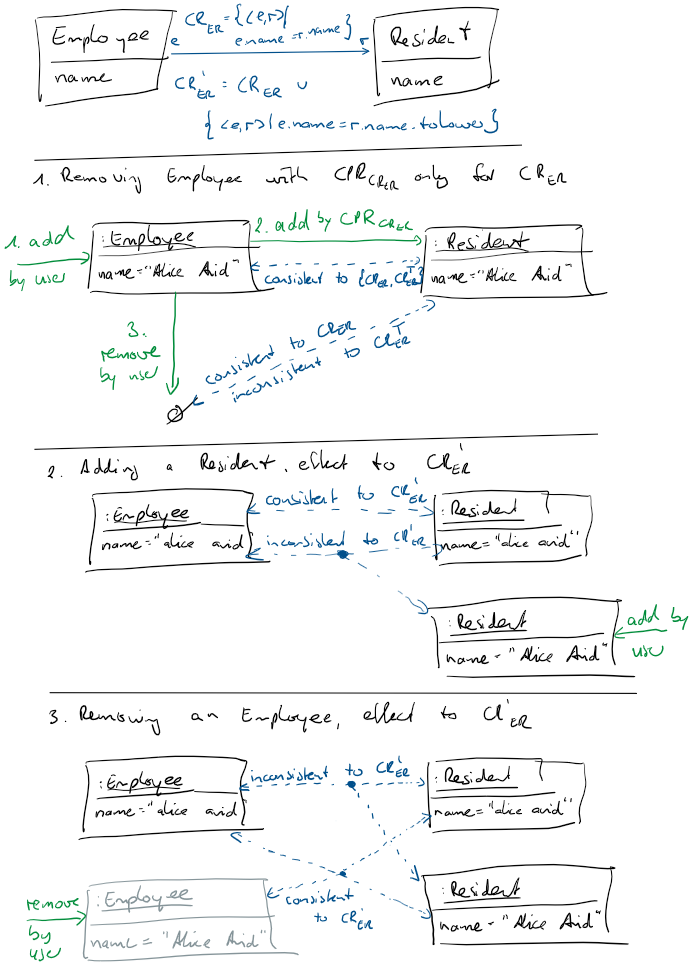
\includegraphics[width=0.87\textwidth]{figures/correctness/synchronization/unidirectional_nonalignment.png}
    \caption[Non-alignment of unidirectional relations and preservation]{Non-alignment of unidirectional relations and preservation rules. Blue lines without arrowheads connect elements that together are consistent or inconsistent to the noted relations. Green lines with arrowheads indicate changes by users or consistency preservation.
    }
    \label{fig:synchronization:unidirectional_nonalignment}
\end{figure}

\mnote{Both relation directions for unidirectional preservation rule}
It is, however, easy to see that a unidirectional consistency preservation rule cannot only consider one direction of consistency relations but needs to consider both.
Consider the example in \autoref{fig:synchronization:unidirectional_nonalignment}, which contains an extract of the consistency relations of the running example.
We assume the consistency relations $\consistencyrelation{CR}{ER}$ and $\consistencyrelation{CR}{ER}^T$ describing that for each employee a single corresponding resident must exist and vice versa.
As discussed before, only considering $\consistencyrelation{CR}{ER}$ would realize the notion of not requiring an employee for every resident.
If we define a unidirectional consistency preservation rule $\consistencypreservationrule{\consistencyrelation{CR}{ER}}$ only for the consistency relation $\consistencyrelation{CR}{ER}$ with the goal to always preserve consistency according to that relation after changes to the employee model, the example scenario 1 in \autoref{fig:synchronization:unidirectional_nonalignment} shows that this is not the case.
The rule properly propagates the change of adding an employee by adding a resident and thus restores consistency.
Removing an employee, however, leads to a violation of consistency.
The removal does not require the consistency preservation rule to perform any changes in the resident model, because $\consistencyrelation{CR}{ER}$ only requires a unique resident to exist for every employee, but does not forbid that there is a resident for which no employee exists.
This is defined by the inverse relation $\consistencyrelation{CR}{ER}^T$.
In consequence, after removing an employee the consistency preservation rule does not perform any changes, as consistency to $\consistencyrelation{CR}{ER}$ is given, but the models are then inconsistent to $\consistencyrelation{CR}{ER}^T$.
$\consistencypreservationrule{\consistencyrelation{CR}{ER}}$ must, however, also be responsible for restoring consistency to $\consistencyrelation{CR}{ER}^T$ in case of an element removal, because the consistency preservation rule $\consistencypreservationrule{\consistencyrelation{CR}{ER}^T}$ for the inverse direction can not restore consistency to $\consistencyrelation{CR}{ER}^T$, as the resident model was not changed.

\mnote{Both relation directions affected by one change}
The given scenario exemplifies the general case that consistency according to a consistency relation cannot only be violated by performing changes to the model containing the left condition elements of the relations, but also by changes to the model containing the right condition elements of the relation.
In general, consistency of models to a consistency relation is affected by the presence of condition elements in the models.
Consistency is defined as the ability to define a witness structure, i.e., a unique mapping between condition elements of the consistency relations that occur in the models.
Thus, adding, changing, or removing elements in a model that constitute a condition element of the consistency relations can lead to inconsistencies.

\mnote{Change type relevance for relation direction}
We can see that every type of change can lead to the violation of a consistency relation in either direction:
\begin{properdescription}
    \item[Addition:] Whenever a condition element of the left side of a consistency relation is added to a model, a corresponding condition element needs to exist in another model. If it does not exist yet, the models are not consistent to that relation.
    When a condition element of the right side of a consistency relation is added to a model, this does, according to the definition of consistency, not require another condition element to exist in another model. It can, however, lead to the situation that no witness structure with a unique mapping between the elements exists anymore.
    Consider the exemplary relation $\consistencyrelation{CR}{ER}'$ in \autoref{fig:synchronization:unidirectional_nonalignment} and the example scenario 2.
    Having an employee with the name \enquote{alice} and a corresponding resident with the same name, the models are consistent to that relation.
    Adding a resident with the name \enquote{Alice} violates $\consistencyrelation{CR}{ER}'$, because the employee \enquote{alice} corresponds to both residents, so there is no mapping inducing a witness structure for consistency.
    In consequence, adding a condition element of the right side of the consistency relation to the models can also violate consistency to a consistency relation.
    \item[Removal:] Whenever a condition element of the right side of a consistency relation is removed from a model, the corresponding condition element in the other model still exists. Because this element does not necessarily have a corresponding one anymore, there may not be a valid witness structure and thus the models may not be consistent anymore.
    When a condition element of the left side of a consistency relation is removed from a model, the originally corresponding element is not connected to the removed element in the witness structure anymore. If there is another element that occurs in a consistency relation pair with that corresponding element, there is no unique mapping of elements anymore.
    Consider again the relation $\consistencyrelation{CR}{ER}'$ in \autoref{fig:synchronization:unidirectional_nonalignment} and the example scenario 3.
    Having two employees and residents with the names \enquote{alice} and \enquote{Alice}, the models are consistent, because each employee has a corresponding resident and vice versa.
    If we remove the employee \enquote{Alice}, the models are not consistent to $\consistencyrelation{CR}{ER}'$ anymore, because the remaining employee corresponds to both residents, so there is no unique mapping between condition elements representing a witness structure.
    \item[Change:] We do not have a precise notion of when a condition element can be considered changed, as elements do not have an identity. 
    Additionally, consistency in terms of being able to find a witness structure is only based on the existence or non-existence of condition elements, thus whether an element was changed or whether it was removed and created makes no difference.
    We might say that a condition element can be considered changed when the change describes modifications of the model elements in the condition element that lead to a new condition element within the same condition.
    This does, conceptually, not differ from the removal of one and the addition of another condition element.
    Thus, the same situations as discussed for addition and removal above can occur.
\end{properdescription}

\mnote{Synchronization of unidirectional preservation rules}
It is also easy to see that there is no trivial way of specifying a unidirectional consistency preservation rule that is synchronizing.
It may seem natural to define a consistency preservation rule that is able to process changes in both models and then return only changes in one of them to restore consistency to close the gap between synchronizing and ordinary transformations.
Consider the situation that we have two residents and employees named \enquote{Alice} and \enquote{Bob}.
If one of them is removed in the residents model and the other in the employees model, then a proper synchronizing transformation should remove both corresponding elements such that the models are empty.
This requires changes to both models.
With a unidirectional consistency preservation rule for each direction, neither of them can produce changes in one of the models that reasonably restore consistency.
Such a rule would necessarily revert one removal to restore consistency, which is not the intended behavior and would probably not be specified by a developer that way.
In consequence, the consistency preservation rule would be undefined for that input, although a synchronization transformation would be able to resolve those changes.
In fact, we would expect to have two unidirectional consistency preservation rules of which each removes one of the elements.
This does, however, violate our existing notion of correctness for a single consistency preservation rule.
In the subsequent sections, we therefore discuss relaxed requirements to unidirectional consistency preservation rules to be able to act like a synchronizing transformation.


%%
%% COMPOSING TWO UNIDIRECTIONAL CPR TO BIDIRECTIONAL TRANSFORMATIONS
%%
\subsection{Bidirectional Transformations}

\mnote{Unidirectional preservation rules for both directions}
A unidirectional consistency preservation rule usually appears in combination with another rule for the opposite direction.
We have seen that even a single unidirectional consistency relation between two metamodels requires unidirectional consistency preservation rules for both directions to preserve consistency according to that relation after changes to instances of either of the metamodels.
Many transformation languages allow the specification of \emph{bidirectional transformations}, which means that they derive unidirectional consistency preservation rules for both directions (see \autoref{chap:foundations:transformations}).

\mnote{Bidirectional transformations}
In general, it is reasonable to consider two unidirectional consistency preservation rules between two metamodels together, such that after changes in instances of any of the two metamodels, the other can be updated to restore consistency.
A synchronizing transformation according to \autoref{def:synchronizingtransformation} is also able to process changes in any of the two models, thus such a notion fits to our goal of emulating synchronizing transformations.
According to common terminology, we define this as a \emph{bidirectional transformation}.

\begin{definition}[Bidirectional Transformation]
    \label{def:bidirectionaltransformation}
    Let $\metamodel{M}{1}$ and $\metamodel{M}{2}$ be two metamodels, and let $\consistencyrelationset{CR}$ be a set of consistency relations between them.
    Additionally, let $\consistencypreservationrule{\consistencyrelationset{CR}}^{\rightarrow}$ and $\consistencypreservationrule{\consistencyrelationset{CR}}^{\leftarrow}$ be unidirectional consistency preservation rules with:
    \begin{align*}
        &
        \consistencypreservationrule{\consistencyrelationset{CR}}^{\rightarrow} : (\metamodelinstanceset{M}{1}, \metamodelinstanceset{M}{2}, \changeuniverse{\metamodel{M}{1}}) \rightarrow \changeuniverse{\metamodel{M}{2}} \cup \setted{\bot} \\
        &
        \consistencypreservationrule{\consistencyrelationset{CR}}^{\leftarrow} : (\metamodelinstanceset{M}{2}, \metamodelinstanceset{M}{1}, \changeuniverse{\metamodel{M}{2}}) \rightarrow \changeuniverse{\metamodel{M}{1}} \cup \setted{\bot}
    \end{align*}
    A \emph{bidirectional transformation} is a triple $\transformation{t} = \tupled{\consistencyrelationset{CR},\consistencypreservationrule{\consistencyrelationset{CR}}^{\rightarrow}, \consistencypreservationrule{\consistencyrelationset{CR}}^{\leftarrow}}$.
\end{definition}

\mnote{Correctness of bidirectional transformations}
We call such a bidirectional transformation correct if both consistency preservation rules are correct according to \autoref{def:unidirectionalconsistencypreservationrulecorrectness}.

\begin{definition}[Bidirectional Transformation Correctness]
    \label{def:bidirectionaltransformationcorrectness}
    Let $\transformation{t} = \tupled{\consistencyrelationset{CR}, \consistencypreservationrule{\consistencyrelationset{CR}}^{\rightarrow}, \consistencypreservationrule{\consistencyrelationset{CR}}^{\leftarrow}}$ be a bidirectional transformation.
    We call $\transformation{t}$ correct if, and only if, $\consistencypreservationrule{\consistencyrelationset{CR}}^{\rightarrow}$ and $\consistencypreservationrule{\consistencyrelationset{CR}}^{\leftarrow}$ are both correct.
\end{definition}

\mnote{Changes of both models}
Such bidirectional transformations ensure that if any of two models is changed, a change for the other is generated such that both changed models are consistent again, or it may fail returning $\bot$.
This does, however, not reflect the case that both models have been modified concurrently, as it is the case in transformation networks and thus supported by our initial definition of synchronizing transformations.
We therefore discuss in the following sections how we can combine the unidirectional consistency preservation rules of a bidirectional transformation and which requirements we have to make to them such that the bidirectional transformation behaves like a synchronizing one.
